\documentclass[11pt, a4paper]{article}
\usepackage[pdftex]{graphicx}	

\linespread{1.1}

\setlength{\oddsidemargin}{41pt}
\setlength{\evensidemargin}{41pt}
\setlength{\textwidth}{515pt}

\setlength{\topmargin}{41pt}
\setlength{\textheight}{733pt}

\setlength{\hoffset}{-1in}
\setlength{\voffset}{-1in}
\setlength{\headheight}{0pt}
\setlength{\headsep}{0pt}

\pagestyle{empty}

\begin{document}
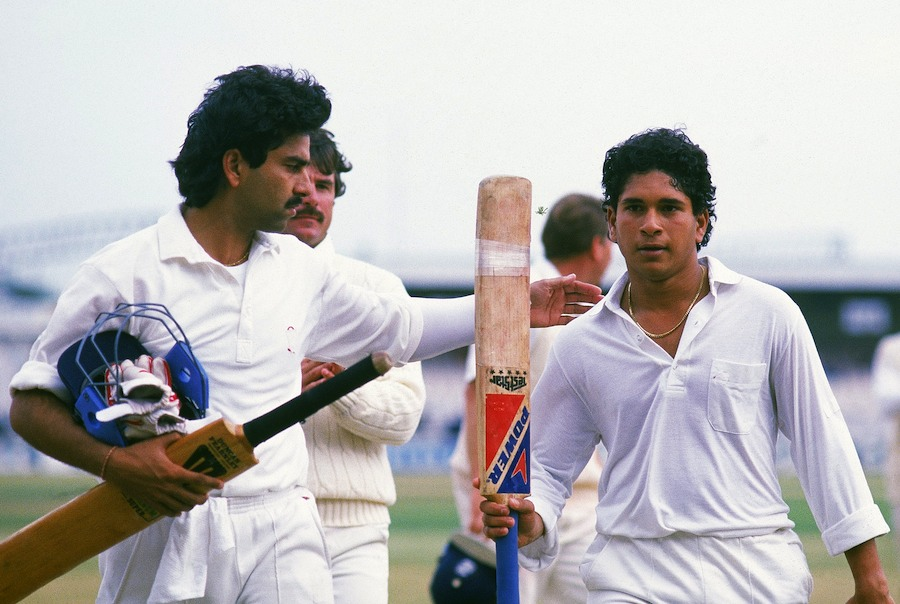
\includegraphics[width=0.9\textwidth]{pics/1.jpg}

Century No.1 

Score: 119* Match: England Vs India 

Series: India in England 1990, 2nd Test 

Venue: Old Trafford, Manchester 

Result: Match drawn 

The first signs of greatness from the Little Master. Sachin Tendulkar's first Test match ton helped India gain a draw from a potentially slippery position. The Manchester ton was the start of many more.
\newpage
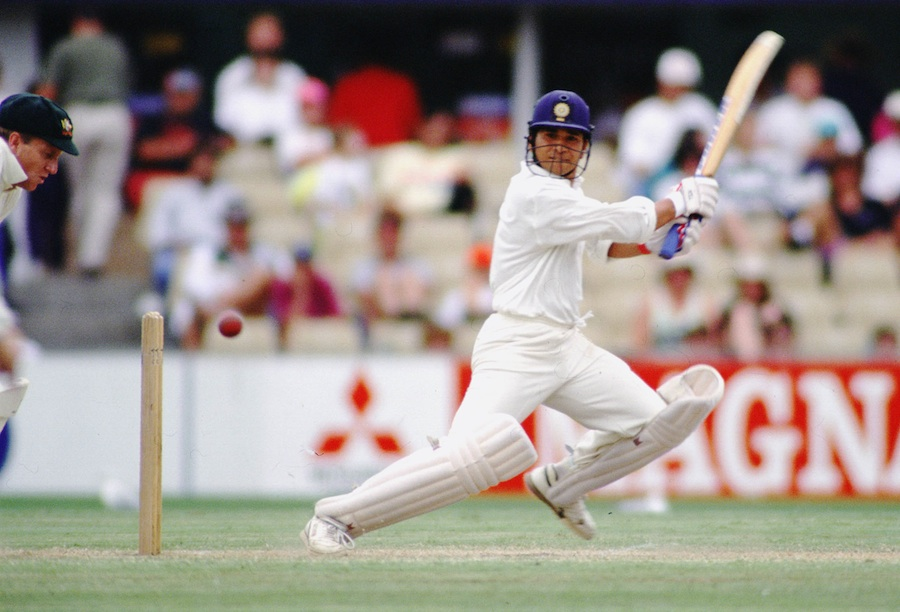
\includegraphics[width=0.9\textwidth]{pics/2.jpg}

Century No.2 

Score: 148* Match: Australia Vs India 

Series: India in Australia 1992, 3rd Test 

Venue: Sydney Cricket Ground 

Result: Match drawn

Tendulkar's reputation as young batting prodigy was swelling. In his first series in Australia, Tendulkar stamped his class scoring two hundreds the first of which arrived in Sydney.
\newpage
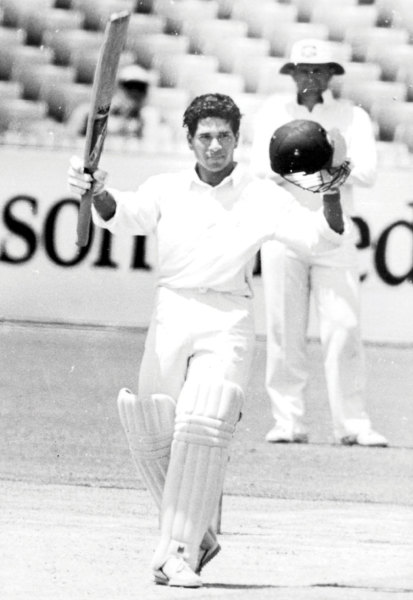
\includegraphics[height=0.8\textheight]{pics/3.jpg}

Century No.3 

Score: 114 

Match: Australia Vs India 

Series: India in Australia 1992, 5th Test 

Venue: WACA, Perth 

Result: Australia won by 38 runs 

When most of the batsmen squirmed away from the bouncers and were unable to cope with the extra pace of the Perth wicket, Tendulkar was a picture of concentration and calm. The knock of 114 runs was a classic, and one which is rated supremely by the little master himself.
\newpage
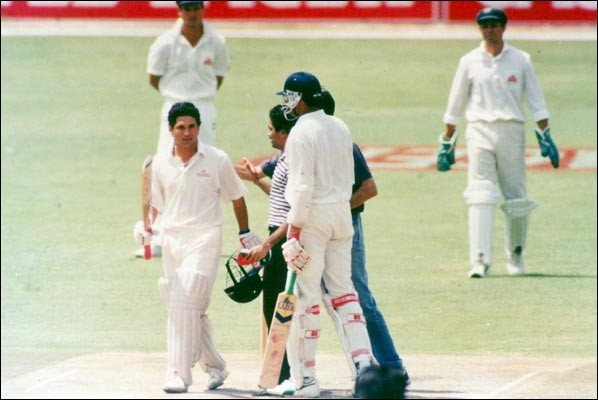
\includegraphics[width=0.9\textwidth]{pics/4.jpg}

Century No.4 

Score: 111 Match: South Africa Vs India 

Series: India in South Africa 1992, 2nd Test 

Venue: New Wanderers Stadium, Johannesburg 

Result: Match drawn 

On a hard and pacy Johannesburg track South Africa led by Allan Donald blew away the Indian batting order. The pace and bounce had all the Indians ducking, weaving and edging, except one--Sachin Tendulkar. India's first innings score read 227, out of which 111 belonged to Tendulkar.
\newpage
\begin{center}
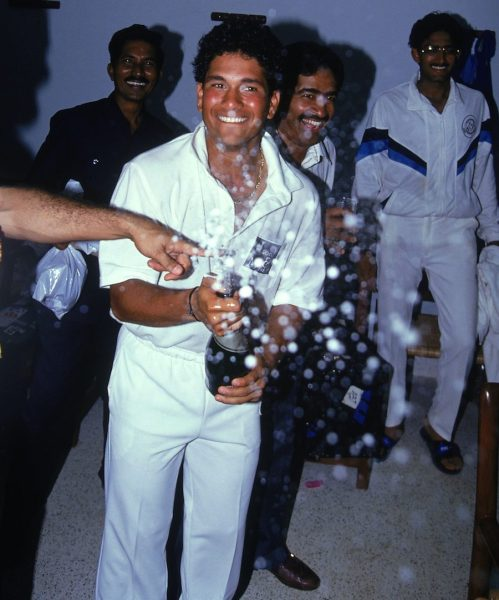
\includegraphics[width=0.6\textwidth]{pics/5.jpg}
\end{center}

Century No.5 

Score: 165 

Match: India Vs England 

Series: England in India 1993, 2nd Test 

Venue: MA Chidambaram Stadium, Chepauk, Madras 

Result: India won by an innings and 22 runs 

England suffered an innings defeat and handed India an unassailable 2-0 lead in the three-match Test series. Batting first, India piled on a total in excess of 500, which largely came off the bat of Tendulkar's masterful 165 runs. This was Sachin's first Test ton on home soil.
\newpage
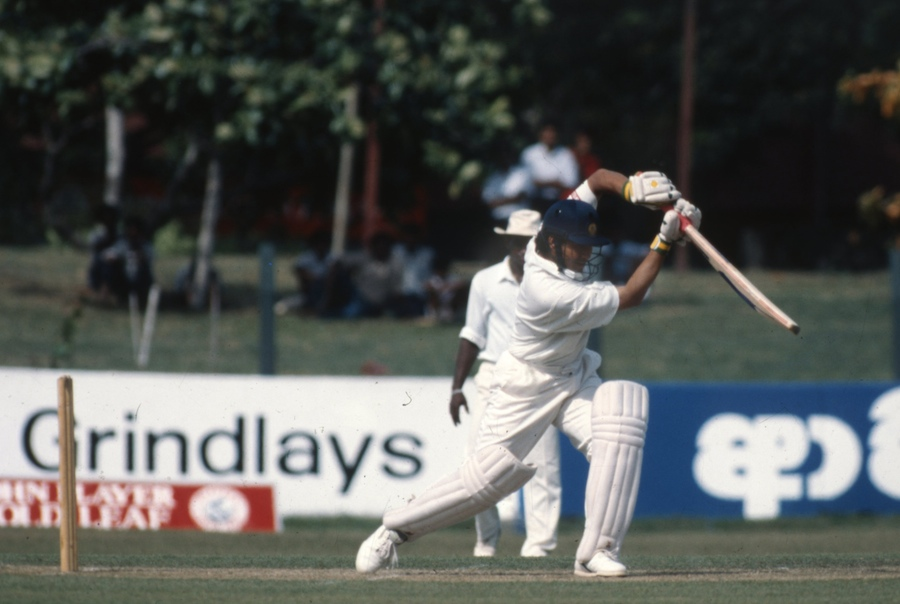
\includegraphics[width=0.9\textwidth]{pics/6.jpg}

Century No.6 

Score: 104* 

Match: India Vs Sri Lanka 

Series: India in Sri Lanka 1993, 2nd Test 

Venue: Sinhalese Sports Club Ground, Colombo 

Result: India won by 235 runs 

An unbeaten century in the second innings helped India set a massive 472-run target against the Lankans. India won the Test handsomely and went on to draw the final game, thereby winning the series 1-0.
\newpage
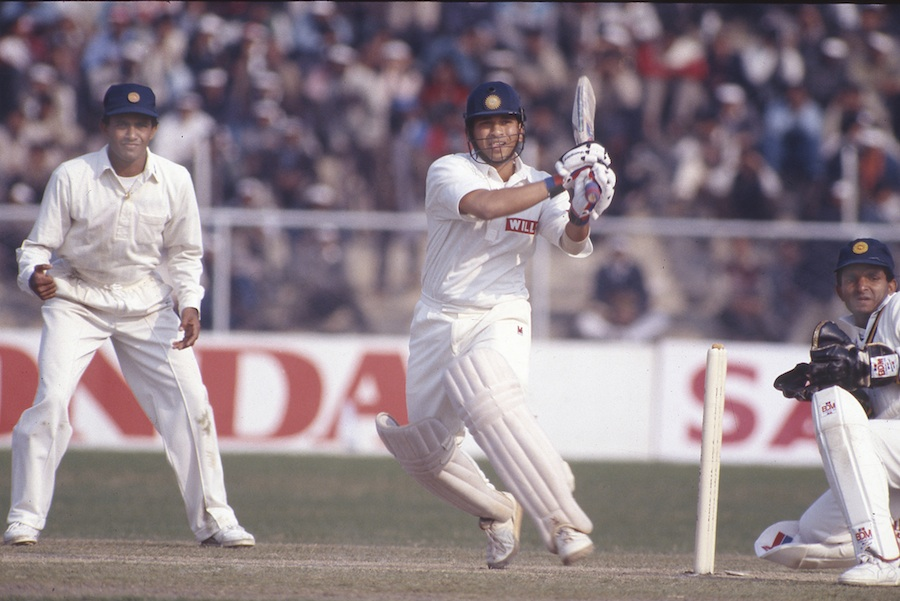
\includegraphics[width=0.9\textwidth]{pics/7.jpg}

Century No.7 

Score: 142 

Match: India Vs Sri Lanka 

Series: Sri Lanka in India 1994, 1st Test 

Venue: KD Singh Babu Stadium, Lucknow 

Result: India won by an innings and 119 runs 

Sachin and India continued to torment Sri Lanka. Tendulkar produced another big ton and the visitors went down by an innings to give India a 1-0 lead in the series.
\newpage
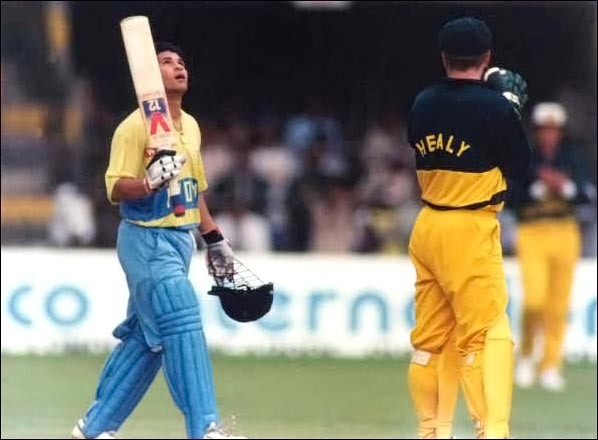
\includegraphics[width=0.9\textwidth]{pics/8.jpg}

Century No.8 

Score: 110 

Series: Singer World Series - 3rd ODI, 1994 

Match: India Vs Australia 

Venue: R Premadasa Stadium, Colombo 

Result: India won by 31 runs 

After seven Test centuries and 78 ODIs, Sachin Tendulkar finally scored his first one-day hundred. The knock came against Australia, an opposition who bore the brunt of Tendulkar's willow in the years to come.
\newpage
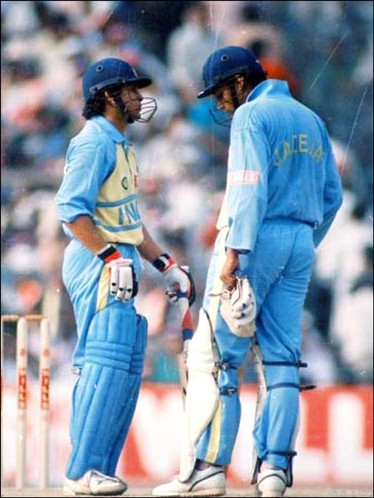
\includegraphics[height=0.8\textheight]{pics/9.jpg}

Century No.9 

Score: 115 

Series: Wills World Series - 3rd ODI, 1994 

Match: India Vs New Zealand 

Venue: IPCL Sports Complex Ground, Baroda 

Result: India won by 7 wickets 

New Zealand racked up 269 runs and soon found out that it was not going to be enough to get them a win. Tendulkar blasted the Kiwi bowlers away and in the end it took a run-out to send him back to the pavilion.
\newpage
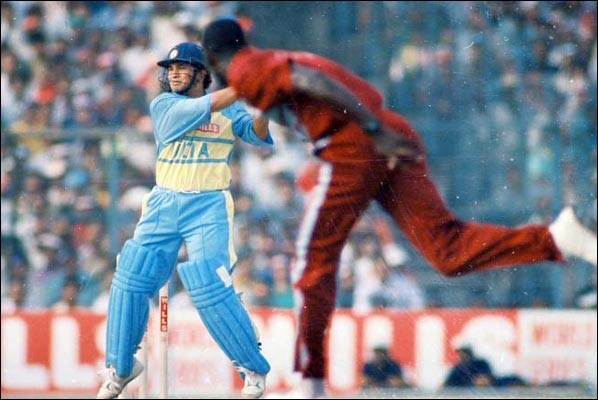
\includegraphics[width=0.9\textwidth]{pics/10.jpg}

Century No.10 

Score: 105 

Series: West Indies in India ODI Series - 5th ODI, 1994 

Match: India Vs West Indies 

Venue: Sawai Mansingh Stadium, Jaipur 

Result: India won by 5 runs 

Tendulkar was declared the Man of the Series scoring over 200 runs in five-match ODI series which India won 4-1. He scored two fifties and registered one century in the series.
\newpage
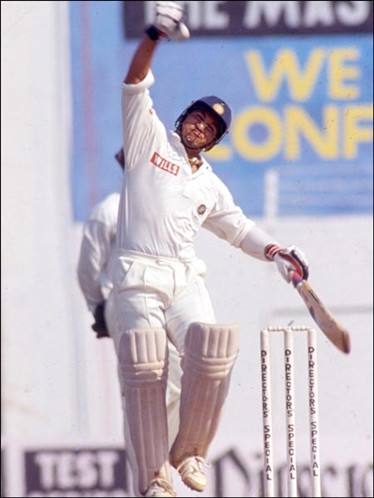
\includegraphics[height=0.8\textheight]{pics/11.jpg}

Century No.11 

Score: 179 

Series: West Indies in India, 2nd Test, 1994 

Match: India Vs West Indies 

Venue: Vidarbha Cricket Association Ground, Nagpur 

Result: Match drawn 

A masterclass from Tendulkar saw India racking up 546 runs in the first innings. The knock was his highest Test score then. Tendulkar brought up his ton with a six off Courtney Walsh.
\newpage
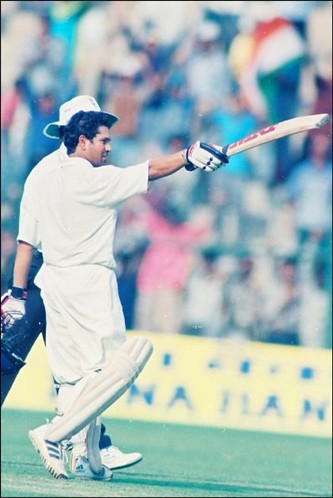
\includegraphics[height=0.8\textheight]{pics/12.jpg}

Century No.12 

Score: 112 

Series: Pepsi Asia Cup - 5th ODI, 1995 

Match: India Vs Sri Lanka 

Venue: Sharjah Cricket Association Stadium 

Result: India won by 8 wickets 

Sri Lanka's target of 203 runs was quickly overhauled by India who were powered by a 107-ball 112 from Tendulkar. His 4th ODI ton was his first at Sharjah.
\newpage
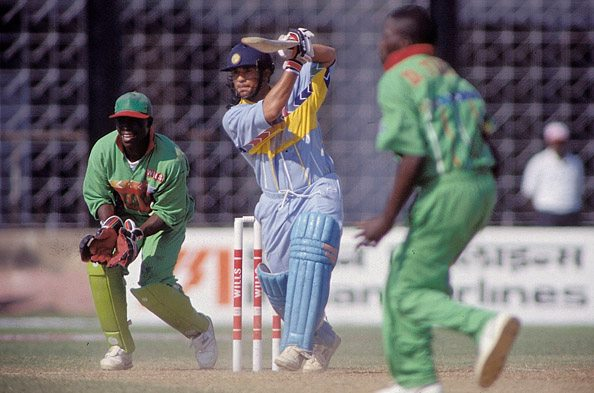
\includegraphics[width=0.9\textwidth]{pics/13.jpg}

Century No. 13 

Score: 127 

Series: Wills World Cup - 6th ODI, Group A, 1996 

Match: India Vs Kenya 

Venue: Barabati Stadium, Cuttack 

Result: India won by 7 wickets 

India and Tendulkar launched their 1996 World Cup campaign in style. The hosts whacked Kenya by 7 wickets and Tendulkar fired his first World Cup hundred.
\newpage
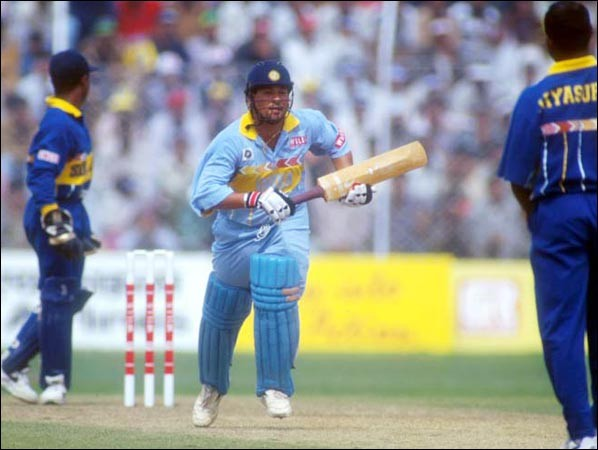
\includegraphics[width=0.9\textwidth]{pics/14.jpg}

Century No. 14 

Score: 137 

Series: Wills World Cup - 24th ODI, Group A, 1996 

Match: India Vs Sri Lanka 

Venue: Feroz Shah Kotla, Delhi 

Result: Sri Lanka won by 6 wickets 

Tendulkar tore apart the Lankan bowlers in a run-a-ball 137. Boundaries flowed from his bat and he smacked eight fours and five sixes. Tendulkar took India to 271 runs, but an inspired Sanath Jayasuriya, whittled away the total with great ease.
\newpage
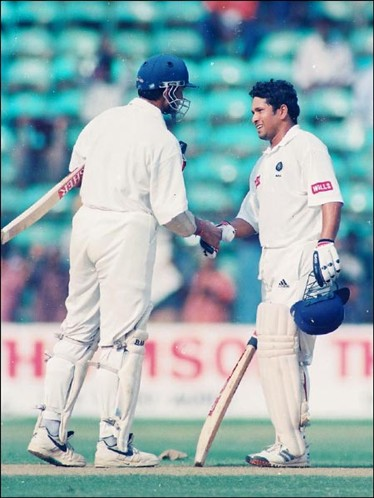
\includegraphics[height=0.8\textheight]{pics/15.jpg}

Century No. 15 

Score: 100 

Series: Singer Cup - 3rd ODI, 1996 

Match: India Vs Pakistan 

Venue: The Padang, Singapore 

Result: Pakistan won by 8 wickets 

Tendulkar's first ODI ton against Pakistan came in losing cause. India was beaten convincingly, and with none of the batsmen sticking out along with Sachin, India was bowled out for 226 runs.
\newpage
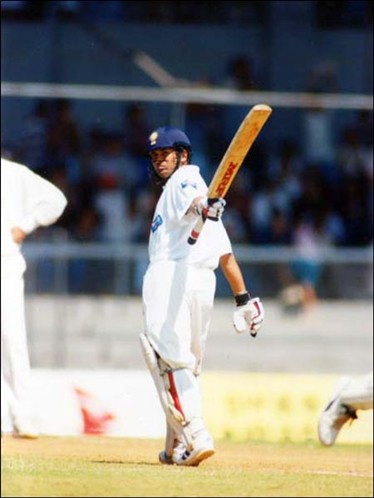
\includegraphics[height=0.8\textheight]{pics/16.jpg}

Century No. 16 

Score: 118 

Series: Pepsi Sharjah Cup - 4th ODI, 1996 

Match: India Vs Pakistan 

Venue: Sharjah Cricket Association Stadium 

Result: India won by 8 wickets 

India got revenge for their bitter defeat in Singapore with a resounding victory in Sharjah. It was the first time India scored 300 runs in a one-day game, with Tendulkar cracking a magnificent ton.
\newpage
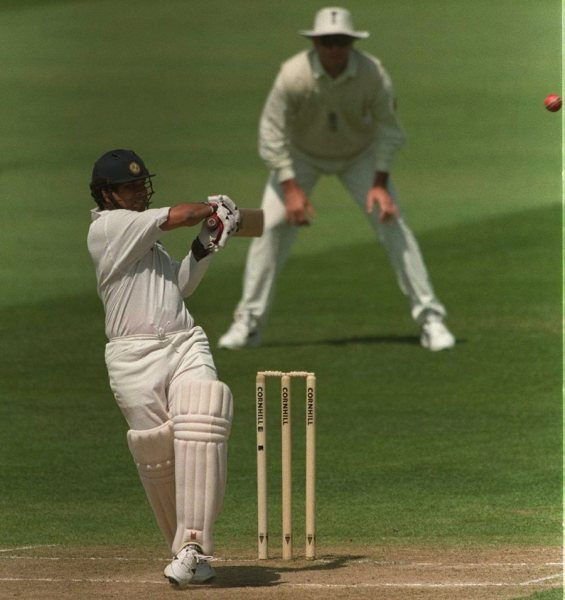
\includegraphics[width=0.9\textwidth]{pics/17.jpg}

Century No. 17 

Score: 122 

Series: India in England 1996, 1st Test 

Match: England Vs India 

Venue: Edgbaston, Birmingham 

Result: England won by 8 wickets 

The burden of India's fragile batting order was once again on the shoulders of Tendulkar who played another gem of a Test knock. While Tendulkar sparkled with a hundred none of the Indian batsmen got past 20 runs.
\newpage
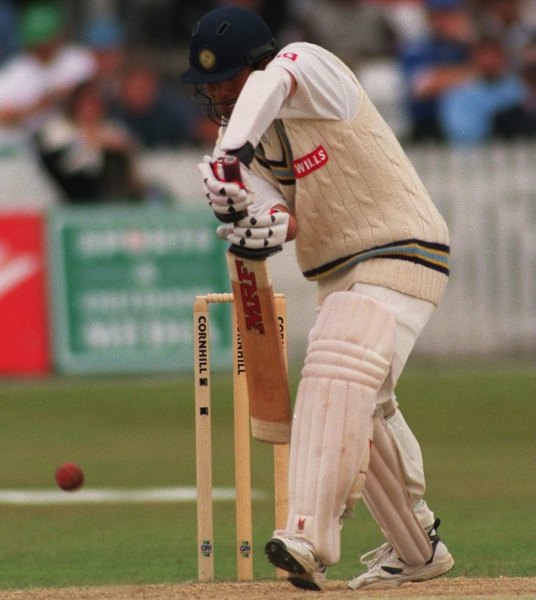
\includegraphics[width=0.9\textwidth]{pics/18.jpg}

Century No. 18 

Score: 177 

Series: India in England 1996, 3rd Test 

Match: England Vs India 

Venue: Trent Bridge, Nottingham 

Result: Match drawn Ganguly and Tendulkar produced great artistry on a slow Nottingham pitch and helped themselves with big centuries. India posted a 500-plus score in the first innings and the match petered out to a draw.
\newpage
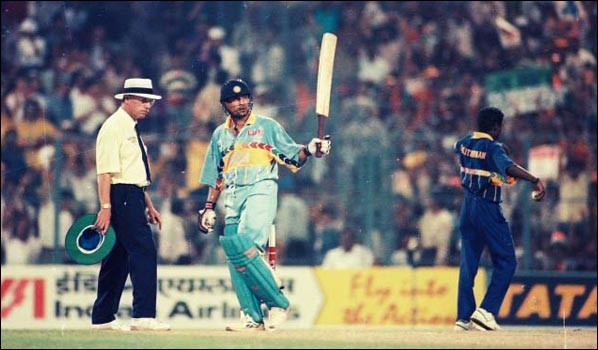
\includegraphics[width=0.9\textwidth]{pics/19.jpg}

Century No. 19 

Score: 110 

Series: Singer World Series - 2nd ODI, 1996 

Match: India Vs Sri Lanka 

Venue: R Premadasa Stadium, Colombo 

Result: Sri Lanka won by 9 wickets 

Tendulkar celebrated his promotion as Indian team's captain with a fluent century at Colombo. Sadly though, the rest of the Indian batting order failed to fire, leaving Tendulkar mulling another ODI defeat.
\newpage
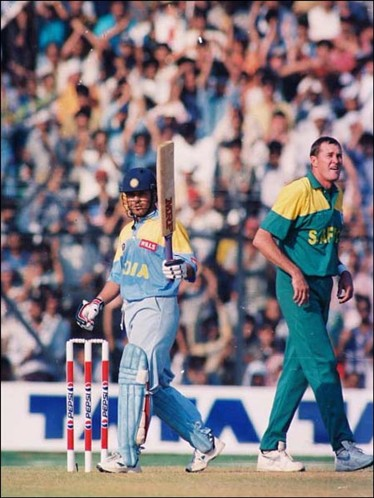
\includegraphics[height=0.8\textheight]{pics/20.jpg}

Century No. 20 

Score: 114 

Series: Mohinder Amarnath Benefit 

Match ODI, 1996 Match: India Vs South Africa 

Venue: Wankhede Stadium, Mumbai 

Result: India won by 74 runs 

After hitting his first ODI ton as the captain of the Indian team, Tendulkar suffered a lean period. The Master though, found his groove with a century against South Africa in a benefit match at his home ground in Mumbai.
\newpage
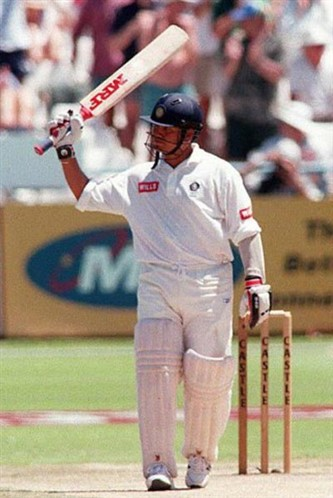
\includegraphics[height=0.75\textheight]{pics/21.jpg}

Century No. 21 

Score: 169 

Series: India in South Africa 1997, 2nd Test 

Match: India Vs South Africa 

Venue: Newlands, Cape Town 

Result: South Africa won by 282 runs 

The visitors were shot out for 100 and 66 in the first Test at Kingsmead, Durban, and a repeat looked well on cards. This until Azhar joined Sachin Tendulkar at the crease. Both the batsmen took on the bowlers and turned the firing the other way. While Azhar played at his carefree best, Sachin was more compact but no less grand.
\newpage
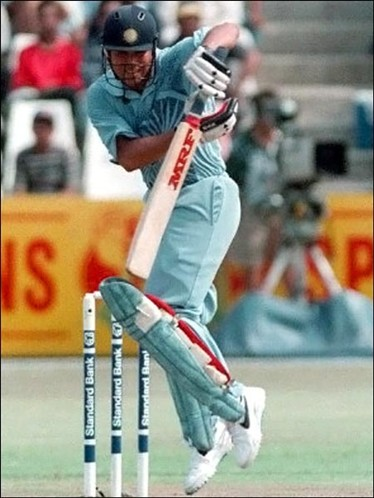
\includegraphics[height=0.8\textheight]{pics/22.jpg}

Century No. 22

Score: 104

Series: Standard Bank International ODI Series - 9th match

Match: India Vs Zimbabwe

Venue: Willowmoore Park, Benoni

Result: India won by 6 wickets

India needed to beat Zimbabwe convincingly and edge past them into the final on the basis of a superior run-rate. With the task cut-out Sachin came out all guns blazing and hammered the Zimbabwe attack.
\newpage
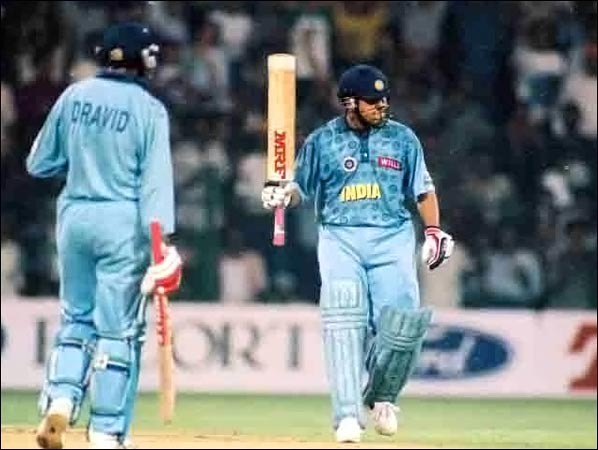
\includegraphics[width=0.9\textwidth]{pics/23.jpg}

Century No. 23

Score: 117

Series: Pepsi Independence Cup - 3rd ODI

Match: India Vs New Zealand

Venue: M Chinnaswamy Stadium, Bangalore

Result: India won by 8 wickets

Tendulkar shook off the blues from a bad tour of South Africa with style against New Zealand in the Independence Cup. He tore into pacer Heath Davis and finished up smacking 117 runs in 137 balls.
\newpage
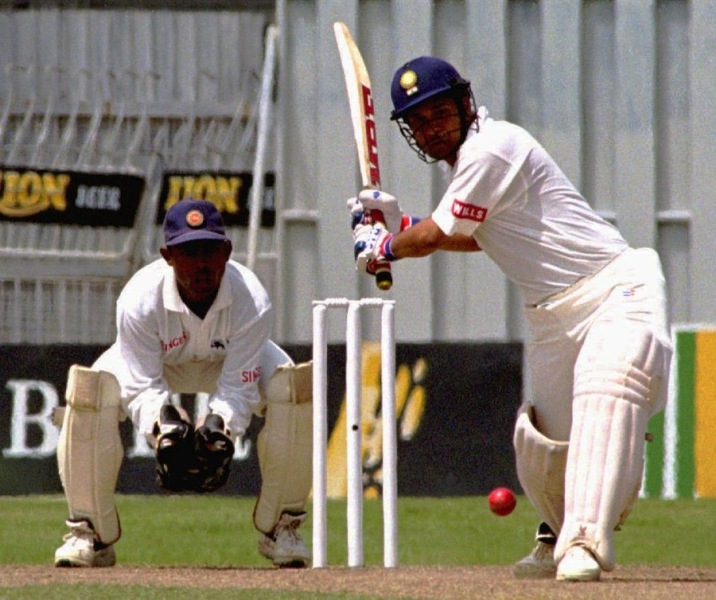
\includegraphics[width=0.9\textwidth]{pics/24.jpg}

Century No. 24

Score: 143

Series: India in Sri Lanka 1997, 1st Test

Match: Sri Lanka Vs India

Venue: R Premadasa Stadium, Colombo

Result: Match drawn

On yet another flat deck in Colombo, Tendulkar helped himself to yet another Test hundred. India piled on 537 and Sri Lanka replied with 952 runs. The scores ensured that the Test's fate ended in a draw.
\newpage
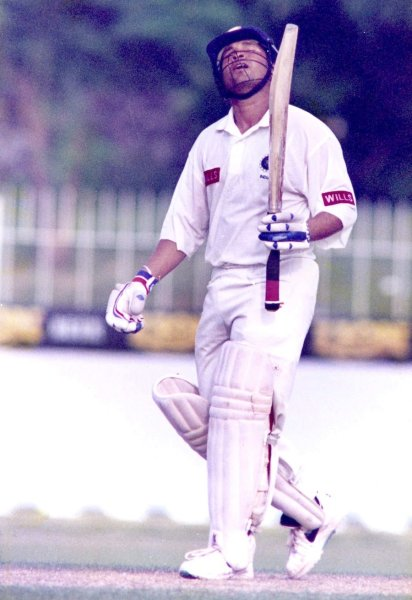
\includegraphics[height=0.8\textheight]{pics/25.jpg}

Century No. 25

Score: 139

Series: India in Sri Lanka 1997, 1st Test

Match: Sri Lanka Vs India

Venue: Sinhalese Sports Club Ground, Colombo

Result: Match drawn

A second successive ton from Sachin and a second successive draw in the series. Sri Lankan wickets played excellent hosts for Indian batsmen and like most of the cricketers, Tendulkar made the most.
\newpage
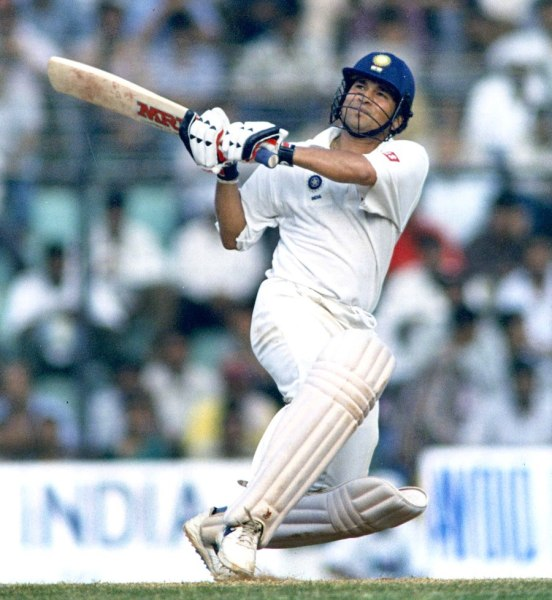
\includegraphics[width=0.9\textwidth]{pics/26.jpg}

Century No. 26

Score: 148

Series: Sri Lanka in India 1997, 3rd Test

Match: India Vs Sri Lanka

Venue: Wankhede Stadium, Mumbai

Result: Match drawn

Tendulkar's 'batathon' continued against Sri Lanka when they had a return tour to India later in the year. The other batsman to shine alongside Tendulkar was Ganguly who scored 173 runs.
\newpage
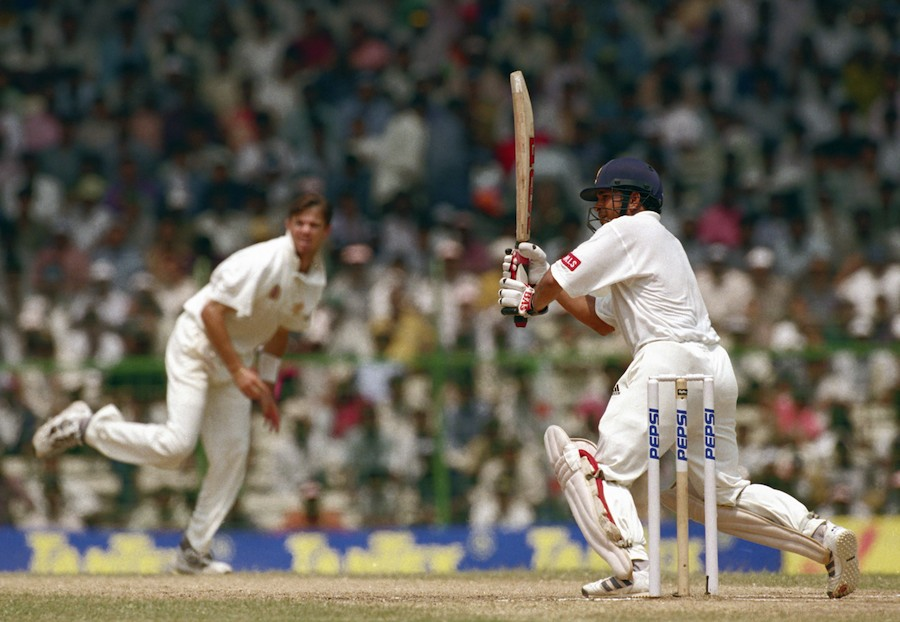
\includegraphics[width=0.9\textwidth]{pics/27.jpg}

Century No. 27

Score: 155*

Series: Australia in India 1998, 1st Test

Match: India Vs Australia

Venue: MA Chidambaram Stadium, Chepauk, Chennai

Result: India won by 179 runs

It was billed as a contest between Shane Warne and Sachin Tendulkar. The Australian leg spinner dismissed Sachin cheaply in the first innings, but in the second the Indian maestro made amends and took the spinner and Australian bowling apart. This Test match saw Sachin deflating Warne by hitting cross-bat shots to balls delivered outside the leg stump.
\newpage
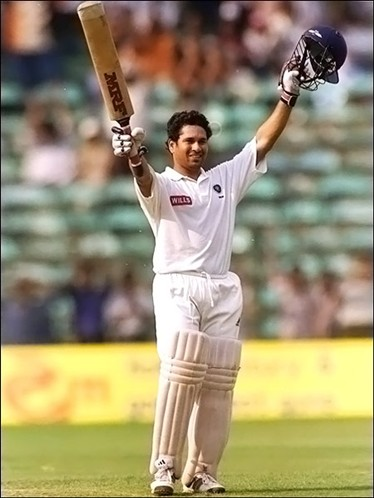
\includegraphics[height=0.8\textheight]{pics/28.jpg}

Century No. 28

Score: 177

Series: Australia in India 1998, 3rd Test

Match: India Vs Australia

Venue: M Chinnaswamy Stadium, Bangalore

Result: Australia won by 8 wickets

Australia continued to suffer at the hands of Sachin Tendulkar who served another masterclass at Bangalore. His second hundred in the series ensured that he scored well above 400-plus runs in the three Test matches.
\newpage
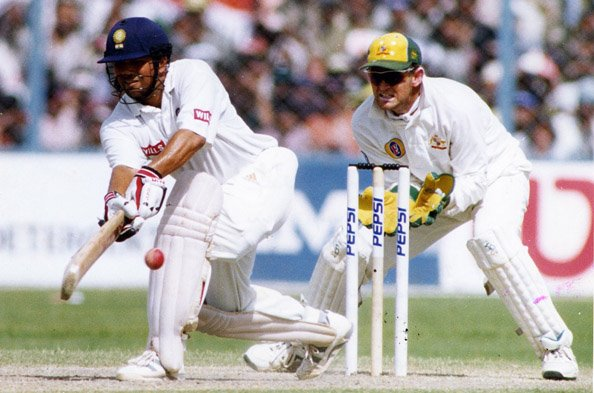
\includegraphics[width=0.9\textwidth]{pics/29.jpg}

Century No. 29

Score: 100

Series: Pepsi Triangular Series - 4th ODI, 1998

Match: India Vs Australia

Venue: Green Park, Kanpur

Result: India won by 6 wickets

Sachin's stronghold over Australia spilled into the ODI series that came after the Test matches. At Green Park, Tendulkar hammered his 13th one-day hundred.
\newpage
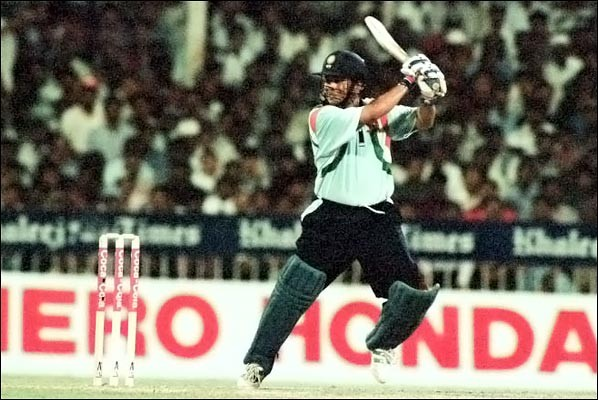
\includegraphics[width=0.9\textwidth]{pics/30.jpg}

Century No. 30

Score: 143

Series: Coca-Cola Cup - 6th ODI, 1998

Match: India Vs Australia

Venue: Sharjah Cricket Association Stadium

Result: Australia won by 26 runs

A classic knock from Tendulkar. One which is most revered by his fans. India needed to win big to edge past New Zealand into the final of the competition. Tendulkar went on a rampage, and despite a dust storm interruption, ensured that India walked into the finals to face Australia once again.
\newpage
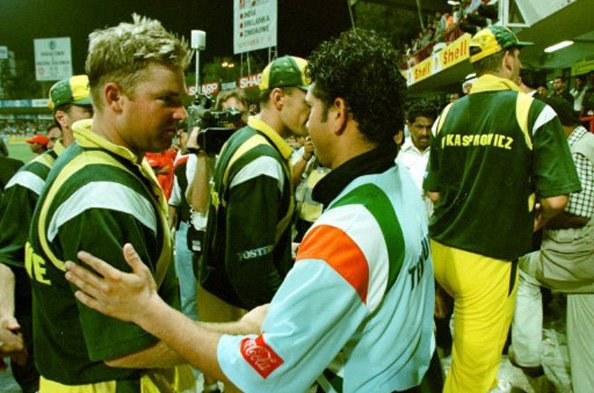
\includegraphics[width=0.9\textwidth]{pics/31.jpg}

Century No. 31

Score: 134

Series: Coca-Cola Cup - final, 1998

Match: India Vs Australia

Venue: Sharjah Cricket Association Stadium

Result: India won by 6 wickets

Within the space of a day, Tendulkar produced another blistering hundred in the final against Australia. It was his 25th birthday and Sachin celebrated it with a match-winning knock.
\newpage
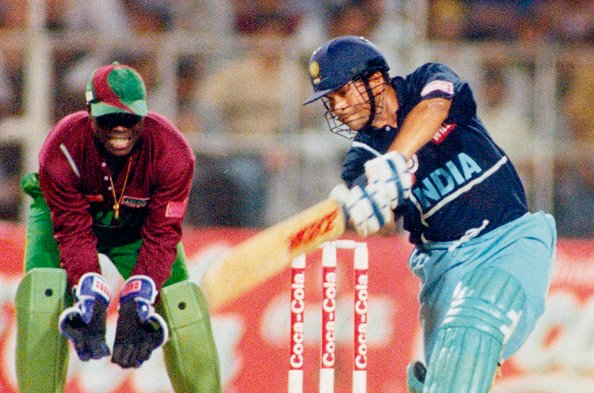
\includegraphics[width=0.9\textwidth]{pics/32.jpg}

Century No. 32

Score: 100*

Series: Coca-Cola Triangular Series - final, 1998

Match: India Vs Kenya

Venue: Eden Gardens, Calcutta

Result: India won by 9 wickets

Another final hundred for Tendulkar. The Kenyans were given a masterclass in one-day batting and India went on to win the match with ease.
\newpage
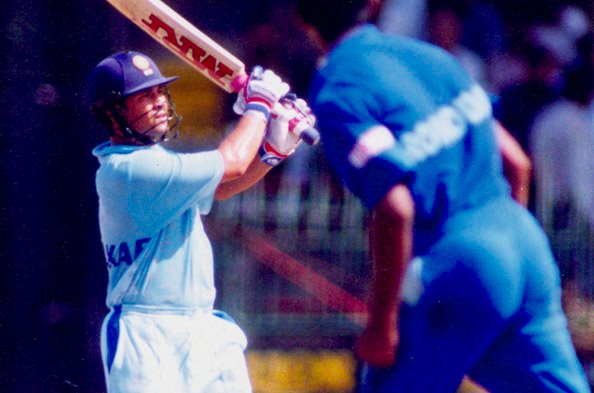
\includegraphics[width=0.9\textwidth]{pics/33.jpg}

Century No. 33

Score: 128

Series: Singer-Akai Nidahas Trophy - final

Match: Sri Lanka Vs India

Venue: R Premadasa Stadium, Colombo

Result: India won by 6 runs

Ganguly and Tendulkar were involved in a record 252-run opening stand. Sachin went past 7000 runs in ODIs and his yet another final ton helped India post a stiff 308-run target against hosts Sri Lanka.
\newpage
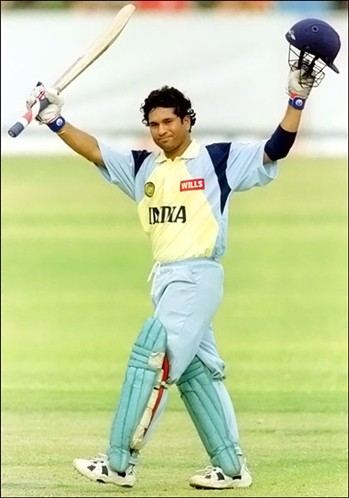
\includegraphics[height=0.8\textheight]{pics/34.jpg}

Century No. 34

Score: 127*

Series: India in Zimbabwe ODI Series 1998 - 1st ODI

Match: Zimbabwe Vs India

Venue: Queens Sports Club, Bulawayo

Result: India won by 8 wickets

India thrashed Zimbabwe comprehensively and Tendulkar smashed his 18th ODI century.
\newpage
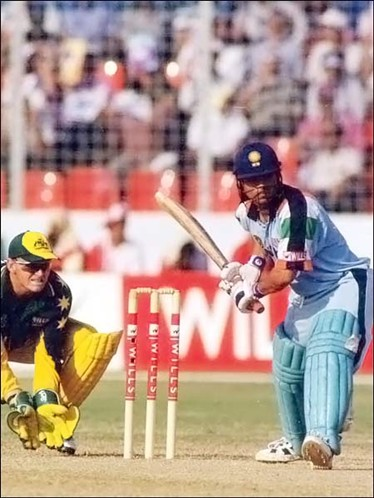
\includegraphics[height=0.8\textheight]{pics/35.jpg}

Century No. 35

Score: 141

Series: Wills International Cup 1998 - 3rd quarter final(Knock-out trophy)

Match: India Vs Australia

Venue: Bangabandhu National Stadium, Dhaka

Result: India won by 44 runs

Tendulkar was all over Australia once again. After India lost quick wickets at the top, Sachin took charge and with the Master in command, India powered to 307 runs. With the ball in his hand in the second innings, Tendulkar tormented Australia further taking 4-38.
\newpage
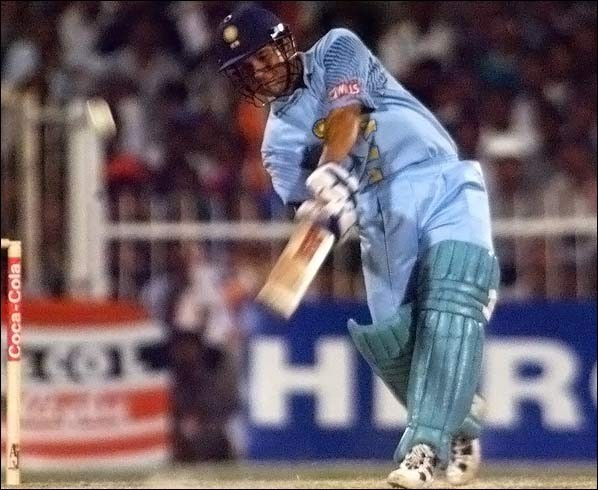
\includegraphics[width=0.9\textwidth]{pics/36.jpg}

Century No. 36

Score: 118*

Series: Coca-Cola Champions Trophy 1998 - 3rd ODI

Match: India Vs Zimbabwe

Venue: Sharjah Cricket Association Stadium

Result: India won by 7 wickets

A target of 197 runs was overhauled with ease with Tendulkar at the helm. He remained unbeaten and guided India home.
\newpage
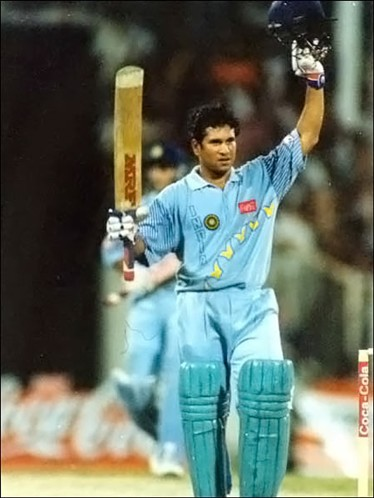
\includegraphics[height=0.75\textheight]{pics/37.jpg}

Century No. 37

Score: 124*

Series: Coca-Cola Champions Trophy 1998 - final

Match: India Vs Zimbabwe

Venue: Sharjah Cricket Association Stadium

Result: India won by 10 wickets

This was the match where Tendulkar famously tore Henry Olonga apart. The bowler had dismissed Sachin with a short delivery in a previous league game and Tendulkar had his revenge blasting the Zimbabwean all over the ground. With a ton in the final Tendulkar became the first batsmen to score twenty international tons.
\newpage
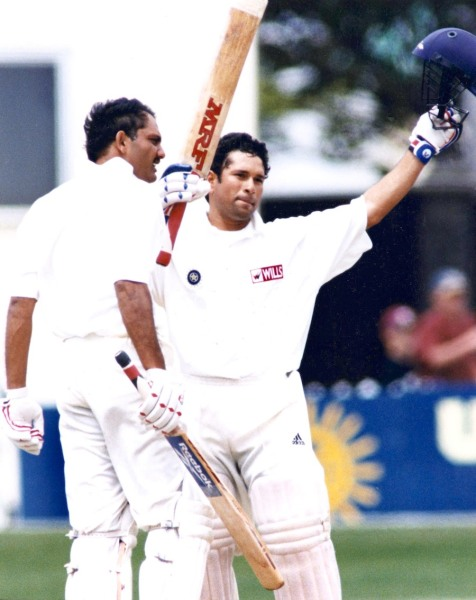
\includegraphics[width=0.8\textwidth]{pics/38.jpg}

Century No. 38

Score: 113

Series: India in New Zealand 1998, 2nd Test

Match: New Zealand Vs India

Venue: Basin Reserve, Wellington

Result: New Zealand won by 4 wickets

A brilliant year for Sachin Tendulkar ended with another glorious century in the second Test. While Azhar mesmerized everyone in the first innings with a breathtaking hundred, Tendulkar sparkled in the second and helped India post a tricky 213-run fourth innings target. New Zealand was 74-5 but Cairns and McMillan made sure the Kiwis would take a 1-0 lead in the series.
\newpage
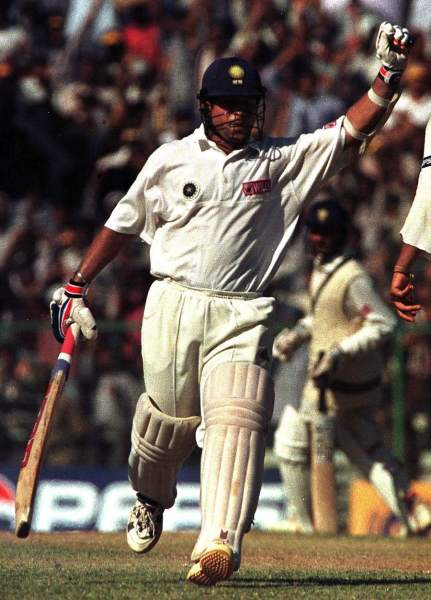
\includegraphics[height=0.75\textheight]{pics/39.jpg}

Century No. 39

Score: 136

Series: Pakistan in India 1999, 1st Test

Match: India Vs Pakistan

Venue: MA Chidambaram Stadium, Chepauk, Chennai

Result: Pakistan won by 12 runs

A tragic hundred from Tendulkar. All hope was lost, and then Mongia and Tendulkar struck a crucial partnership, bringing India close to Pakistan's target. Fighting a bad back and incisive bowling from the likes of Wasim, Waqar and Saqlain Mustaq, Tendulkar fell when India were 17 runs short of the target. India lost the match by 12 runs.
\newpage
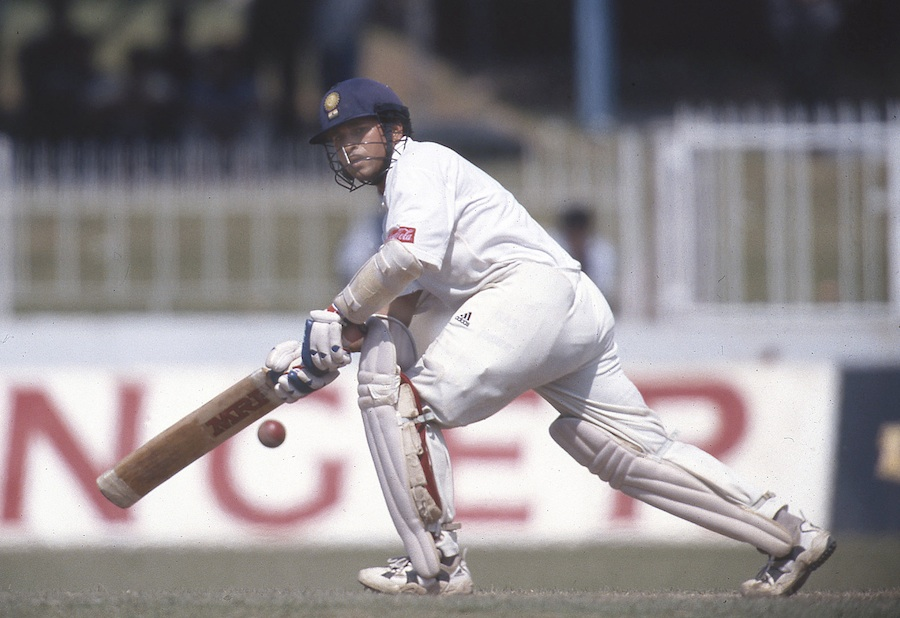
\includegraphics[width=0.9\textwidth]{pics/40.jpg}

Century No. 40

Score: 124*

Series: Asian Test Championship 1999 - 2nd Test

Match: Sri Lanka Vs India

Venue: Sinhalese Sports Club Ground, Colombo

Result: Match drawn

Another Test match in Sri Lanka played on yet another batting beauty, saw Sachin help himself to another Test match hundred. The experimental Asian Test Championship was eventually won by Pakistan.
\newpage
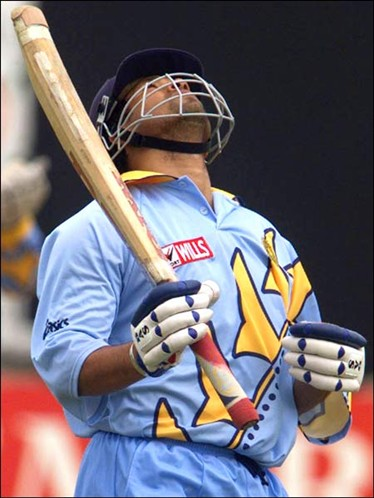
\includegraphics[height=0.8\textheight]{pics/41.jpg}

Century No. 41

Score: 140*

Series: ICC World Cup 1999 - 15th ODI, Group A

Match: India Vs Kenya

Venue: County Ground, Bristol

Result: India won by 94 runs

An emotional century from Tendulkar, who came back to play a memorable knock just days after losing his father.
\newpage
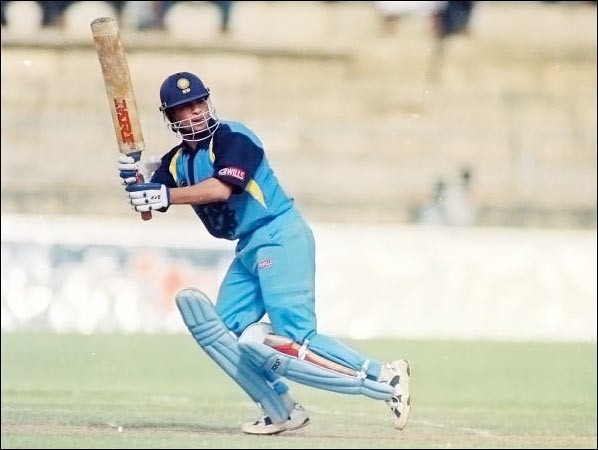
\includegraphics[width=0.9\textwidth]{pics/42.jpg}

Century No. 42

Score: 120

Series: Aiwa Cup 1999 - 6th ODI

Match: Sri Lanka Vs India

Venue: Sinhalese Sports Club Ground, Colombo

Result: India won by 23 runs(D/L method)

After a disappointing World Cup campaign in England, Tendulkar replaced Azhar as the captain of the Indian team. With the burden of captaincy on his shoulders, Sachin fired 23rd ODI ton.
\newpage
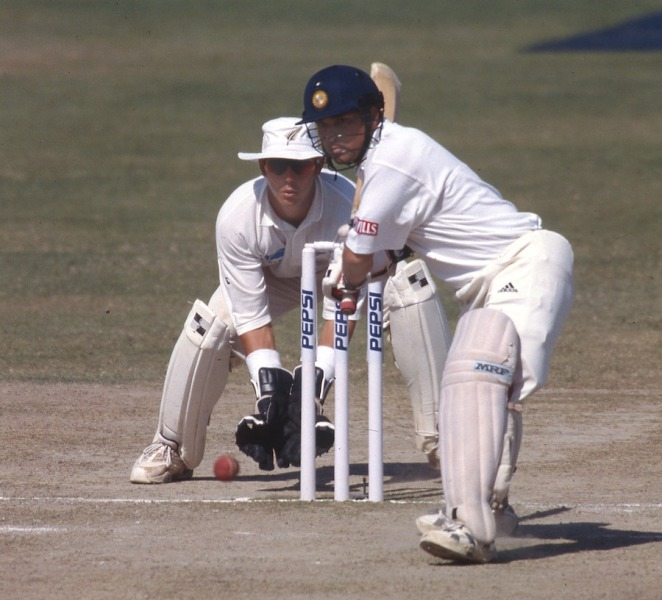
\includegraphics[width=0.9\textwidth]{pics/43.jpg}

Century No. 43 

Score: 126* 

Series: New Zealand in India 1999, 1st Test 

Match: India Vs New Zealand 

Venue: PCA Stadium, Mohali, Chandigarh 

Result: Match drawn 

India was shot out for 83 in the first innings, but came back with a vengeance in the second. Led by Sachin Tendulkar's unbeaten 126 and Dravid's 144, India made sure the game faded into a draw.
\newpage
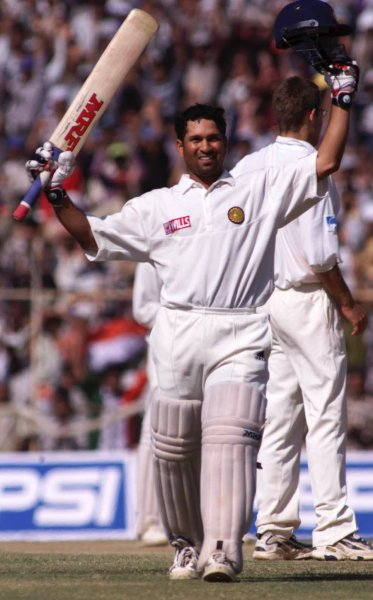
\includegraphics[height=0.8\textheight]{pics/44.jpg}

Century No. 44 

Score: 217 

Series: New Zealand in India 1999, 3rd Test 

Match: India Vs New Zealand 

Venue: Sardar Patel Stadium, Motera, Ahmedabad 

Result: Match drawn 

A grinding innings from Tendulkar saw India posting 500-plus score in their first innings. The knock was Tendulkar's second double in Test matches. 
\newpage
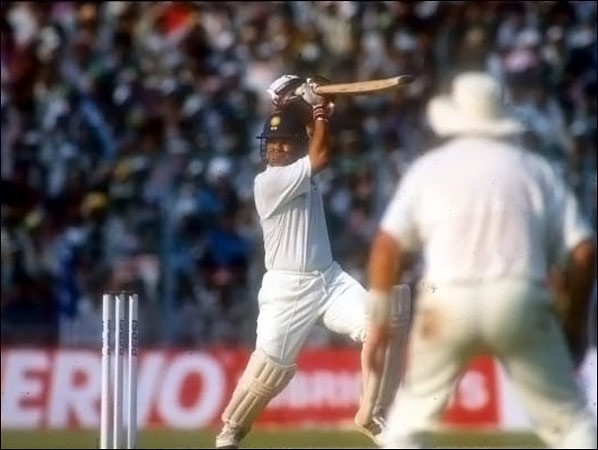
\includegraphics[width=0.9\textwidth]{pics/45.jpg}

Century No. 45 

Score: 186* 

Series: New Zealand in India 1999, 2nd ODI 

Match: India Vs New Zealand 

Venue: Lal Bahadur Shastri Stadium, Hyderabad, Deccan 

Result: India won by 174 runs 

An exhilarating knock which sent the Kiwi bowlers in a tizzy. The rocket-paced innings contained 20 boundaries and three sixes.
\newpage
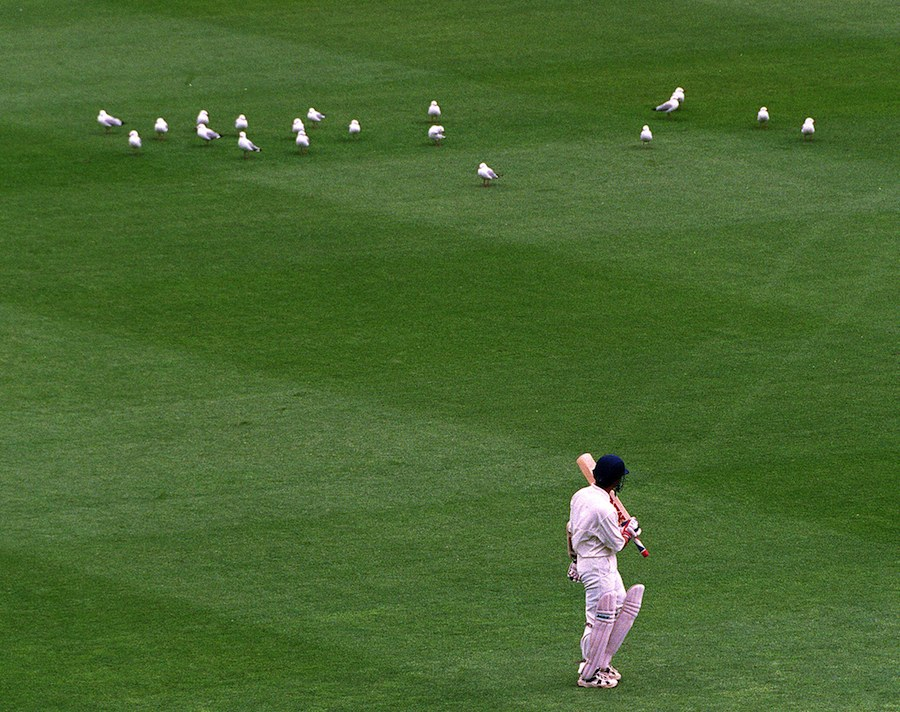
\includegraphics[width=0.9\textwidth]{pics/46.jpg}

Century No. 46 

Score: 116 

Series: Border-Gavaskar Trophy 1999 - 2nd Test 

Match: Australia Vs India 

Venue: Melbourne Cricket Ground 

Result: Australia won by 180 runs 

India was in their familiar backs to the wall situation in the second Test when Tendulkar arrived in the middle and played a majestic knock. His Melbourne hundred was his only ton in the series where India was thrashed 3-0 in the Test series and won just a solitary ODI in the triangular contest alongside Pakistan.
\newpage
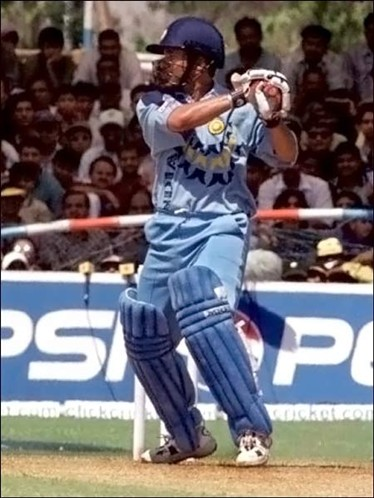
\includegraphics[height=0.8\textheight]{pics/47.jpg}

Century No. 47 

Score: 122 

Series: South Africa in India ODI Series 2000 - 4th ODI 

Match: India Vs South Africa 

Venue: IPCL Sports Complex Ground, Vadodara 

Result: India won by 4 wickets 

After suffering a torrid series in Australia Tendulkar relinquished the captaincy. In the ODI series that followed the Test series, Tendulkar shone with a knock of 122 runs and helped chase down a stiff 
283-run target to give India an unbeatable 3-1 lead in the series.
\newpage
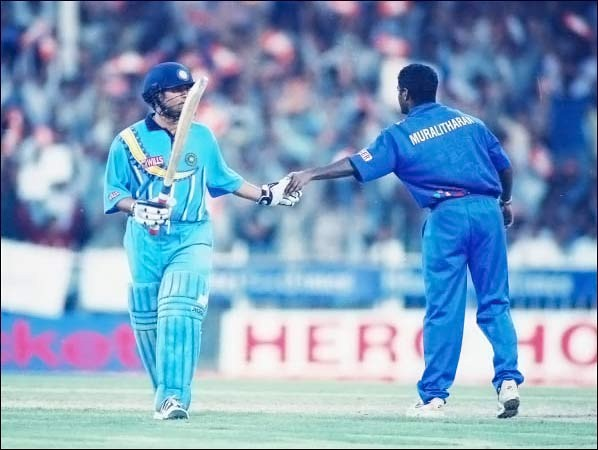
\includegraphics[width=0.9\textwidth]{pics/48.jpg}

Century No. 48 

Score: 101 

Series: Coca-Cola Champions Trophy - 1st ODI 

Match: India Vs Sri Lanka 

Venue: Sharjah Cricket Association Stadium 

Result: Sri Lanka won by 5 wickets 

Tendulkar produced another Sharjah hundred, but inevitably it came in yet another losing cause for India. It was his 26th ton in ODIs.
\newpage
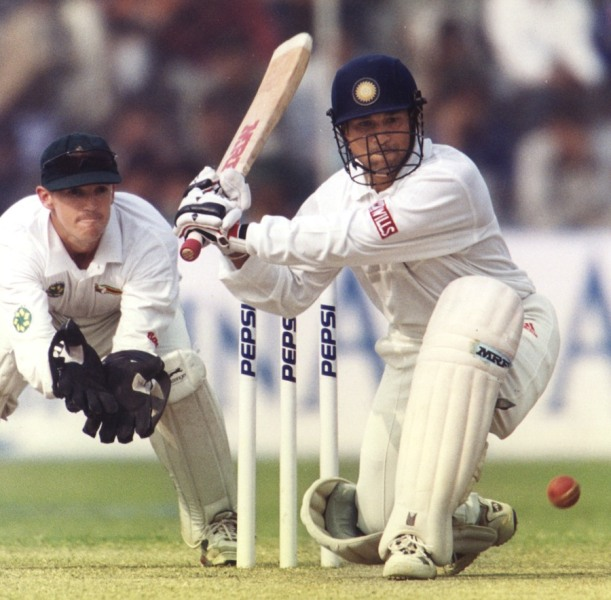
\includegraphics[width=0.9\textwidth]{pics/49.jpg}

Century No. 49 

Score: 122 

Series: Zimbabwe in India Test Series 2000 - 1st Test 

Match: India Vs Zimbabwe 

Venue: Feroz Shah Kotla, Delhi 

Result: India won by 7 wickets 

Rahul Dravid scored his first double in Tests and Sachin ended with only his second Test century against Zimbabwe. Captain Ganguly made a bold declaration and India completed a comprehensive win.
\newpage
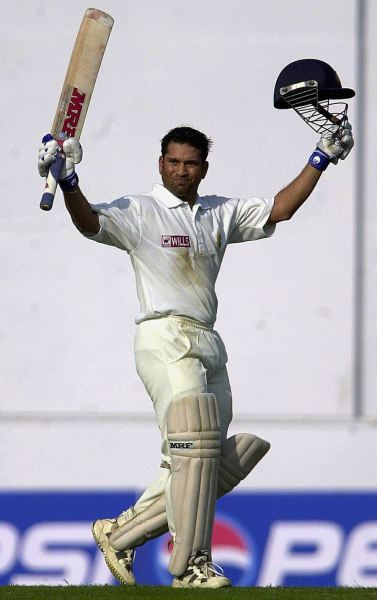
\includegraphics[height=0.8\textheight]{pics/50.jpg}

Century No. 50 

Score: 201* 

Series: Zimbabwe in India Test Series 2000 - 2nd Test 

Match: India Vs Zimbabwe 

Venue: Vidarbha Cricket Association Ground, Nagpur 

Result: Match drawn 

Tendulkar's fiftieth international century went on to become his second double hundred in Test matches.
\newpage
\includegraphics[height=0.8\textheight]{pics/51.jpg}

Century No.51 

Score: 146 

Series: Bilateral ODI series, 2000 

Match: India V Zimbabwe, 3rd ODI 

Venue: Jodhpur 

Result: Zimbabwe won by 1 wicket 

The brilliant 146 by the Little Master was filled with 17 hits to the fence and propelled India to 284 in their 50 overs. This was later overshadowed by a magnificent partnership between the Flower brothers for Zimbabwe, who chased down the target with 1 ball to spare and 1 wicket in hand.
\newpage
\includegraphics[width=0.9\textwidth]{pics/52.jpg}

Century No.52 

Score: 126 

Series: Border-Gavaskar Trophy, 2001 

Match: India V Australia, 3rd test 

Venue: Chennai 

Result: India won by 2 wickets 

This match was in many ways an exhibition of test cricket. The series was levelled 1-1 before the Chennai test and when Australia put up 391 in their first innings thanks to Mathew Hayden's double hundred, they were in a very strong position. All this changed once Sachin came out to bat and scored a majestic 126 to help India surpass the 500-run mark. India never really looked back from there and despite a lion-hearted effort by Jason Gillespie, India won the match by 2 wickets.
\newpage
\includegraphics[width=0.9\textwidth]{pics/53.jpg}

Century No.53 

Score: 139 

Series: Bilateral ODI series, 2001 

Match: India V Australia, 3rd ODI 

Venue: Indore 

Result: India won by 118 runs 

After losing the second ODI at Pune by a fairly wide margin, India bounced back to take the lead at Indore's Nehru Stadium. Propelled by Sachin's 139 that came off just 125 balls with 19 fours, India amassed 299. That target was always going to be difficult for the Aussies, who folded up for just 181.
\newpage
\includegraphics[width=0.9\textwidth]{pics/54.jpg}

Century No.54 

Score: 122 

Series: 2001 tri-series in Zimbabwe featuring Zimbabwe, India and West Indies 

Match: India V West Indies, 6th match of preliminary stage 

Venue: Harare 

Result: India won by 6 wickets 

This match was seen as a dress rehearsal before the final as both India and West Indies had already booked their place in the summit clash. Indian bowlers had done a very good job of restricting the West Indies to a less-than-competitive 229 in their allotted 50 overs. Buoyed by a brisk opening stand of 133 between Sachin and Ganguly, India made the task look easy. Sachin went to score his century at a run-a-ball and guide India to a comfortable win.
\newpage
\includegraphics[width=0.9\textwidth]{pics/55.jpg}

Century No.55 

Score: 101 

Series: 2001 tri-series in South Africa featuring India, South Africa and Kenya 

Match: India V South Africa, 1st match of the tournament 

Venue: Johannesburg 

Result: South Africa won by 6 wickets 

It was a thrilling start to the tri-series as India put up a respectable 279 on a good batting wicket at the Wanderers. It could have been a lot higher had the Indian middle order capitalised on a great start provided by Ganguly and Sachin. Both the openers scored centuries and enjoyed a partnership of 193 in just 35 overs. Ironically, South Africa then rode on Sachin's 'guru' to reach 280 with nearly 2 overs to spare. Gary Kirsten made a wonderful 133.
\newpage
\includegraphics[width=0.9\textwidth]{pics/56.jpg}

Century No.56 

Score: 146 

Series: 2001 tri-series in South Africa featuring India, South Africa and Kenya 

Match: India V Kenya, 9th match of the tournament 

Venue: Paarl 

Result: India won by 186 runs 

It was a stroll in the park at Paarl for India. For the second time in the tri-series, Indian openers both scored centuries and this time their partnership went much higher. The duo put on 258 for the first wicket and Sachin scored 146. Kenya was no match while chasing a mammoth 351 and gave up the chase in the early stages itself to end their tally at 165 for 5.
\newpage
\includegraphics[width=0.9\textwidth]{pics/57.jpg}

Century No.57 

Score: 155 

Series: Bilateral test series, 2001 

Match: India V South Africa, 1st test 

Venue: Bloemfontein 

Result: South Africa won by 9 wickets 

India blew up a golden opportunity to do well in an overseas test after two top batsmen got wonderful centuries. Virender Sehwag made 105 coming down the batting order while Sachin, in his usual no.4 position crafted a majestic 155 off just 184 balls to pulverise the Proteas' bowling attack. With 23 fours and 1 six, Sachin took India to a decent 379 in the first essay. South Africa responded with centuries from Lance Klusener and Hershelle Gibbs to make sure they were always ahead in the test. They chased down a modest 54 to win the test by 9 wickets and take a 1-0 lead in the series.
\newpage
\includegraphics[width=0.9\textwidth]{pics/58.jpg}

Century No.58 

Score: 103 

Series: Bilateral test series, 2001 

Match: India V England , 2nd test 

Venue: Ahmedabad 

Result: Match drawn 

It was a very patient knock by the little master on a fairly difficult track and under pressure. England had batted first at Motera and notched up a competitive 407 with very useful contributions coming from batsmen down the order. Indian batsmen struggled against the left-arm spin of Ashley Giles but Sachin ensured the damage would be limited. His knock took so much time off the test that England couldn't press home for a win. India retained their 1-0 lead.
\newpage
\includegraphics[width=0.9\textwidth]{pics/59.jpg}

Century No.59 

Score: 176 

Series: Bilateral test series, 2002 

Match: India V Zimbabwe, 1st test 

Venue: Nagpur 

Result: India won by an innings and 101 runs 

After back-to-back tough series' against South Africa and England, India has an easy summer with Zimbabwe. The first test was played at the Vidarbha Cricket Association Ground (the old one) on a fairly dull track. Zimbabwe were bundled out for 287 and India responded with a 176 from Sachin and centuries from SS Das and Sanjay Bangar to make 570 for 7. What followed was a mere formality for Indian bowlers.
\newpage
\includegraphics[height=0.7\textheight]{pics/60.jpg}

Century No.60 

Score: 117 

Series: Bilateral series, 2002 

Match: India V West Indies, 2nd test 

Venue: Port of Spain, Trinidad 

Result: India won by 37 runs 

India went in to the Caribbean series with serious hope after a decent tour of South Africa just the year before. They were getting closer and closer to getting rid of that tag of tigers only at home. This Indian team, under the leadership of Sourav Ganguly was gradually emerging as a fearless bunch on overseas soil. The first test at Guyana was drawn and India played their second test at one of their favourite venues in the West Indies, Port of Spain. Sachin's splendid century in the first innings took India to a reasonable 339. Although the West Indies won large parts of second innings, India emerged triumphant.
\newpage
\includegraphics[width=0.9\textwidth]{pics/61.jpg}

Century No.61 

Score: 105 N.O. 

Series: 2002 Tri-series in England featuring India, England and Sri Lanka 

Match: India V England, 5th match of the tournament 

Venue: Chester-le-Street 

Result: No result 

India had begun the tri-series with a bang by beating both England and Sri Lanka in their opening fixtures. Then came this day-night clash at Chester-le-Street. India won the toss and decided to leave the chasing to England. Sachin and Yuvraj blasted the hapless English bowling attack to all parts of the ground on their way to a staggering 170-run partnership. Sachin eased his way to 105 and remained not out at the end of 50 overs. England's chase was halted in the 13th over by the weather Gods and that was it. No result. 
\newpage
\includegraphics[width=0.9\textwidth]{pics/62.jpg}

Century No.62 

Score: 113 

Series: 2002 Tri-series in England featuring India, England and Sri Lanka 

Match: India V Sri Lanka, 9th match of the tournament 

Venue: 

Result: India won by 63 runs 

Barely a week after he caressed English bowlers at Chester-le-Street, Sachin was in ominous touch again. This time, it was against the Lankans. He smashed 113 off just 102 balls to help India surge past the 300-run mark and that did the trick. The Lankans did put up some resistance but it was a case of too-little-too-late from them.
\newpage
\includegraphics[width=0.9\textwidth]{pics/63.jpg}

Century No.63 

Score: 193 

Series: Bilateral test series, 2002 

Match: India V England, 3rd test 

Venue: Headingly 

Result: India won by an innings and 46 runs 

This has to rank among the greatest test victories for India on two counts. First, it came in difficult overseas conditions in England and second, it came when they had their backs to the wall. India notched up 628 for 8 in their first innings with centuries from Dravid, Sachin and Ganguly. The trio never needed to bat again in the test match as Kumble \& Co finished off England twice to inflict an innings defeat.
\newpage
\includegraphics[width=0.9\textwidth]{pics/64.jpg}

Century No.64 

Score: 176 

Series: Bilateral test series, 2002 

Match: India V West Indies, 3rd test 

Venue: Kolkata 

Result: Match drawn 

India had already won the test series 2-0 coming in to the final test at Eden Gardens. West Indies, by taking a handy first innings lead of 139 runs put tremendous pressure on India. At one stage, India was reduced to 87 for 4 in the second innings. This is when Sachin and Laxman came together and punctured West Indies hopes once and for all. Sachin's match-saving knock lasted 7 hours and was laced with 26 superb hits to the fence.
\newpage
\includegraphics[height=0.75\textheight]{pics/65.jpg}

Century No.65 

Score: 152 

Series: World Cup 2003 

Match: India V Namibia, Pool A fixture 

Venue: Pietermaritzburg 

Result: India won by 181 runs 

India had come into this Pool A fixture after a drubbing only a week ago at the hands of defending champions Australia. Against Namibia, it was always going to be an easy outing for India but the question was how easy. The famous ODI combo of Sachin and Ganguly came to the party again with a stand of 244 for the second wicket (Sehwag had started opening by then). Sachin's 152 had 18 hits to the fence and interestingly none over it.
\newpage
\includegraphics[height=0.7\textheight]{pics/66.jpg}

Century No.66 

Score: 100 

Series: 2003 Tri-series featuring India, Australia and New Zealand 

Match: India V Australia, 2nd match of the tournament 

Venue: Gwalior 

Result: India won by 37 runs 

India versus Australia was beginning to gain momentum ever since the two sides clashed in the World Cup final the same year in South Africa. In this clash, India had lost Sehwag in the very first over to Nathan Bracken. Sachin and Laxman then steadied the ship with a 190-run partnership for the second wicket. Both batsmen got centuries and helped India reach a commanding 283 from their 50 overs. Australia was in the hunt with Gilchrist getting a quickfire 83 but once he departed, it was India all the way. Sachin also picked up a wicket. 
\newpage
\includegraphics[height=0.7\textheight]{pics/67.jpg}

Century No.67 

Score: 102 

Series: 2003 Tri-series featuring India, Australia and New Zealand 

Match: India V New Zealand, 9th match of the tournament 

Venue: Hyderabad 

Result: India won by 145 runs 

Lal Bahadur Shastri stadium is easily one of Sachin's favourite venues. Back in 1999, Sachin had killed the kiwi bowling at the same venue on his way to a great knock of 186. And here he was again against the same opponent. This time, it was a lot lesser than 186 since Sehwag was keen to steal the limelight with his 130. Nonetheless, Sachin's century and his opening wicket stand of 182 with Viru took India to a comfortable 145-run over New Zealand.
\newpage
\includegraphics[height=0.75\textheight]{pics/68.jpg}

Century No.68 

Score: 241 N.O. 

Series: Border-Gavaskar Trophy, 2004 

Match: India V Australia, 4th test 

Venue: Sydney 

Result: Match drawn 

It was an epic clash at the SCG and it had an epic performance from an epic cricketer. Sachin Tendulkar blasted his first hundred of the series and what a knock it was. It helped India shatter many records while racing to 705 for 7 against the mighty Aussies. It needed a combination of poor umpiring and gritty Steve Waugh to ensure Australia would walk away with a draw. Sachin's knock was laced with 33 hits to the boundary and lasted more than 10 hours. What concentration!
\newpage
\includegraphics[width=0.9\textwidth]{pics/69.jpg}

Century No.69 

Score: 141 

Series: Bilateral ODI series, 2004 

Match: India V Pakistan, 2nd ODI 

Venue: Rawalpindi 

Result: Pakistan won by 12 runs 

Three days after winning a nail-biter at Lahore, India came into the second ODI at Pindi with confidence on a high. The bowlers allowed that to be punctured somewhat with ordinary effort as Pakistan batsmen, led by top order piled up 329 in 50 overs. India responded in style with Sachin leading from the front with a solid 141. Sachin's knock came from just 135 balls and put India on course for a great win until the middle order failed to come up with the goods. India ended 12 short.
\newpage
\includegraphics[width=0.9\textwidth]{pics/70.jpg}

Century No.70 

Score: 194 

Series: Bilateral test series, 2004 

Match: India V Pakistan, 1st test 

Venue: Multan 

Result: India won by an innings and 52 runs 

This was an out and out Sehwag match, which is why very few remember Sachin's performance in this historic clash. Many Indian teams had travelled to Pakistan over the years but none could actually inflict massive defeats on the Pakistanis. Sehwag scored his maiden triple century and Sachin 194 as India piled up 675 in their first innings. Sachin was actually unbeaten when captain Dravid decided to declare. There was a lot of hue and cry that followed. Many were unhappy with Dravid for not giving Sachin a chance to complete his double century.
\newpage
\includegraphics[width=0.9\textwidth]{pics/71.jpg}

Century No.71 

Score: 248 N.O. 

Series: Bilateral test series, 2004 

Match: India V Bangladesh, 1st test 

Venue: Dhaka 

Result: India won by an innings and 140 runs 

After a great tour down under exactly a year ago, India was increasingly establishing itself as world beaters not just at home but even on overseas surfaces. Bangladesh was always going to be easy meat for the red-hot Indian team. Expectedly, the series began in a one-sided manner. Bangladesh was bundled out for just 184 and Indian then piled on the misery with very good batting display. Sachin smashed an unbeaten 248 as the team scored 526 and pushed the local boys to the corner. Bangladesh was bundled out for just 202 in its second essay. Sachin's 248 came from nearly 10 hours and had 35 classy hits to the fence.
\newpage
\includegraphics[width=0.9\textwidth]{pics/72.jpg}

Century No.72 

Score: 123 

Series: Bilateral ODI series, 2005 

Match: India V Pakistan, 4th ODI 

Venue: Ahmedabad 

Result: Pakistan won by 3 wickets 

The series was well poised after India won the first match at Vizag and Pakistan responded with a win at Jamshedpur. India won the toss and batted first. Sachin blasted 123 off 130 balls as India raced to 315, which on most surfaces is a match-winning one. Pakistan had other ideas though with almost everyone at the top of the order contributing their bit. It was a close contest but the men from across the border emerged triumphant.
\newpage
\includegraphics[height=0.75\textheight]{pics/73.jpg}

Century No.73 

Score: 109 

Series: Bilateral test series, 2005 

Match: India V Sri Lanka, 2nd test 

Venue: Delhi 

Result: India won by 188 runs 

Sachin was the lone centurion in the test, which was in the balance for long periods before India marched ahead in the late stages. India depended on Sachin's patient 109 (took 5 hours) to muster 290 in their first essay. Sri Lanka failed to capitalise on a good start to their chase and collapsed from 175 for 2 to just 230 all out. That turned the match on its head and India finished as the winning side.
\newpage
\includegraphics[width=0.9\textwidth]{pics/74.jpg}

Century No.74 

Score: 100 

Series: Bilateral ODI series, 2006 

Match: India V Pakistan, 1st ODI 

Venue: Peshawar 

Result: Pakistan won via D/L method 

After the roaring success of the 2004 tour of Pakistan, the 2006 one was rather difficult for the Indian team. They struggled in the test series but it was a different story in the shorter format. Sachin got a century in the first ODI but India failed to defend 305 from 47 overs. But, the team went on to win the remaining four ODIs in the series to wrap it up 4-1.
\newpage
\includegraphics[width=0.9\textwidth]{pics/75.jpg}

Century No.75 

Score: 141 N.O. 

Series: Tri-series in Kuala Lumpur featuring India, Australia and West Indies 

Match: India V West Indies, 2nd match of the tournament 

Venue: Kuala Lumpur 

Result: West Indies won via D/L method 

It was one of those occasions when Sachin carried the bat through the 50 overs of an ODI inning. He made 141 from 148 balls with 13 fours and 5 towering 6s on a smallish Kinrara Academy Oval ground. Fidel Edwards and Dwayne Bravo were punished severely by the little master. West Indies began their response in style with Chris Gaye smashing 45 off 35 balls. When the weather Gods intervened, the Windies were comfortably ahead on Duckworth Lewis method.
\newpage
\includegraphics[width=0.9\textwidth]{pics/76.jpg}

Century No.76 

Score: 100 N.O. 

Series: Bilateral ODI series, 2007 

Match: India V West Indies, 4th ODI 

Venue: Vadodara 

Result: India won by 160 runs 

Prior to this game, it was a closely contested ODI series with India winning the first two matches by 14 and 20 runs respectively while the Windies won the 3rd ODI by 3 wickets. It all changed though at Vadodara. India hammered the Windies bowling attack to make a commanding 341 in 50 overs with Sachin becoming the lone centurion scoring exactly a hundred. The Caribbeans were never really in the hunt and eventually folded up for 181 in the 42nd over.
\newpage
\includegraphics[width=0.9\textwidth]{pics/77.jpg}

Century No.77 

Score: 101 

Series: Bilateral test series, 2007 

Match: India V Bangladesh, 1st test 

Venue: Chittagong 

Result: Match drawn 

It was a rain-hit test match where India called the shots for long periods but lack of time made a result impossible. India batted first and made 387 with centuries from Sachin and Ganguly. Sachin's inning was a painstaking effort lasting nearly 5 hours. It was very unlike Sachin but who cares. It is the end number that matters in cricket.
\newpage
\includegraphics[height=0.75\textheight]{pics/78.jpg}

Century No.78 

Score: 122 N.O. 

Series: Bilateral test series, 2007 

Match: India V Bangladesh, 2nd test 

Venue: Mirpur 

Result: India won by an innings and 239 runs 

If weather Gods saved Bangladesh in the first test, the next one at Mirpur exposed the gap between Bangladesh and the rest of test-playing nations. It wasn't just a defeat. It was an embarrassment for the Bangladeshis. The top four batsmen in the batting order for India all scored centuries and that included Sachin's unbeaten 122. The combined first and second innings totals of Bangladesh still fell short of follow on par score of 410!
\newpage
\includegraphics[width=0.9\textwidth]{pics/79.jpg}

Century No.79 

Score: 154 N.O. 

Series: Border-Gavaskar Trophy, 2008 

Match: India V Australia, 2nd test 

Venue: Sydney 

Result: Australia won by 122 runs 

Sachin's magnificent 154 came as a like-for-like for Andrew Symonds' double hundred, which had propelled Australia to 463 in the first innings. The Master Blaster's knock took India to 532 and a handy first innings lead of 69 runs. Sachin's 154 came in 7 hours and had 14 fours and 1 six. Then came the remarkable turnaround by the Aussies who amassed 401 in just 107 second innings overs leaving India with a target of 333. The 'triple nelson' haunted the Indians as they folded up for 210.
\newpage
\includegraphics[height=0.7\textheight]{pics/80.jpg}

Century No.80 

Score: 153 

Series: Border-Gavaskar Trophy, 2008 

Match: India V Australia, 4th test 

Venue: Adelaide 

Result: Match drawn 

India had come into the final test at Adelaide Oval after registering one of their greatest test victories ever. On what is perceived as the fastest wicket in the world, India beat Australia at Perth to get 
themselves a chance of squaring the series at Adelaide. And their mission began on a sound note with Sachin hammering 153 from just 205 balls (Incredibly fast for test cricket) and India reached 526. Australian batsmen though lived up to their billing and ensured they walked away with a draw in the match and win in the series.
\newpage
\includegraphics[height=0.7\textheight]{pics/81.jpg}

Century No.81 

Score: 117 N.O. 

Series: 2008 tri-series in Australia featuring India, Australia and Sri Lanka 

Match: 1st Final: India V Australia 

Venue: Sydney 

Result: India won by 6 wickets 

For all those who questioned Sachin's temperament on big occasions, this inning served as the perfect response from the little master. Chasing 240 to take a crucial lead in the best-of-three finals, Sachin played right through the chase to help India ease past the 240-mark with 4 overs remaining. The fact that Sachin's 117 only had 10 hits to the fence just shows how calculated his whole approach was. 
\newpage
\includegraphics[width=0.9\textwidth]{pics/82.jpg}

Century No.82 

Score: 109 

Series: Border-Gavaskar Trophy, 2008 

Match: India V Australia, 4th test 

Venue: Nagpur (Jamtha) 

Result: India won by 172 runs 

For a change, it was a completely one-sided test series between India and Australia as the kangaroos struggled to cope with transition. Coming into the final test at Jamtha, Nagpur, India held a slender 1-0 lead and the Aussies were desperate to show there was life in them after all. Any hope the Aussies nourished was soon punctured when India notched up 441 in the first innings thanks to a great century by Sachin.
\newpage
\includegraphics[height=0.75\textheight]{pics/83.jpg}

Century No.83 

Score: 103 

Series: Pataudi Trophy, 2008 

Match: India V England, 1st test 

Venue: Chennai 

Result: India won by 6 wickets 

This was easily one of the most special moments for Sachin in his career. The India-England series had been abruptly called off following the 26/11 Mumbai blasts and when it resumed after a month, Sachin wanted to do something special. He did so in style. India chased down a mammoth 387 in the final inning thanks to great unbeaten 103 by the little master at one of his favourite venues. 
\newpage
\includegraphics[width=0.9\textwidth]{pics/84.jpg}

Century No.84 

Score: 163 retired hurt 

Series: Bilateral ODI series, 2009 

Match: India V New Zealand, 3rd ODI 

Venue: Christchurch 

Result: India won by 58 runs 

AMI Stadium under lights always presents a fascinating sight to the eye and when someone like Sachin Tendulkar goes tearing apart the bowlers, it just adds to the glitz and excitement. Sachin was at his imperious best on the day and it was unfortunate he had to retire hurt on 163 with still 5 overs left. The world record and maybe even double hundred was within his sights. India made 392 and New Zealand played well but not well enough as they folded up for 334 in 45 overs.
\newpage
\includegraphics[width=0.9\textwidth]{pics/85.jpg}

Century No.85 

Score: 160 

Series: Bilateral test series, 2009 

Match: India V New Zealand, 1st test 

Venue: Hamilton 

Result: India won by 10 wickets 

It is not often that a team from the sub-continent goes to New Zealand and beats the Kiwis. This Indian team was different. It was full of aggressive cricketers who no more feared the overseas surfaces. New Zealand batted first at Hamilton and made 279. India responded with 520 thanks to Sachin's 160, which had 26 majestic hits to the fence. Trailing by 241, New Zealand fought gallantly in the second essay but were no match to the tough Indians.
\newpage
\includegraphics[width=0.9\textwidth]{pics/86.jpg}

Century No.86 

Score: 138 

Series: 2009 tri-series in Sri Lanka featuring India, Sri Lanka and New Zealand 

Match: Final: India V Sri Lanka 

Venue: Colombo (Premadasa) 

Result: India won by 46 runs 

A year after he guided India to a title triumph in Australia, Sachin took India to another title win. This time, it was in Sri Lanka in the final of tri-series. Batting first after winning the toss, India put up 319 on the board thanks to 138 by Sachin. The Little Master's knock was laced with 10 fours and 1 six. The Lankans fought hard but folded up 46 runs short.
\newpage
\includegraphics[height=0.75\textheight]{pics/87.jpg}

Century No.87 

Score: 175 

Series: Bilateral ODI series, 2009 

Match: India V Australia, 5th ODI 

Venue: Hyderabad (Rajiv Gandhi stadium) 

Result: Australia won by 3 runs 

Chasing down an improbable 351, India fought all the way through and was even ahead of the Aussies at many stages during the chase. This was largely due to Sachin's magnificent inning of 175 where he single-handedly demolished the Aussie bowling attack. The sad part was he got out just when he shouldn't have and India lost momentum to eventually lose the match by just 3 runs.
\newpage
\includegraphics[width=0.9\textwidth]{pics/88.jpg}

Century No.88 

Score: 100 N.O. 

Series: Bilateral test series, 2009 

Match: India V Sri Lanka, 1st test 

Venue: Ahmedabad 

Result: Match drawn 

It was a match-saving effort from Sachin in a test where most things went wrong for India. The bowlers had conceded a record 760 at home against the Lankans and then had their backs to the wall while trying to avoid the prospect of innings loss. Sachin played out five hours for his century and kept the Lankans spin attack led by Muttiah Muralitharan at bay.
\newpage
\includegraphics[height=0.8\textheight]{pics/89.jpg}

Century No.89 

Score: 105 N.O. 

Series: Bilateral test series, 2010 

Match: India V Bangladesh, 1st test 

Venue: Chittagong 

Result: India won by 113 runs 

Sachin was a lone warrior in a very poor Indian batting effort in the first innings. The Little master scored 105 in an Indian 1st innings effort of 243. India made amends in the second innings to make 413 to win the match by a handsome margin. Sachin's brilliant 105 in the first essay came in just 166 balls.
\newpage
\includegraphics[width=0.9\textwidth]{pics/90.jpg}

Century No.90 

Score: 143 

Series: Bilateral test series, 2010 

Match: India V Bangladesh, 2nd test 

Venue: Mirpur 

Result: India won by 10 wickets 

Days after scoring a wonderful century to help India to respectability at Chittagong, Sachin came up with the goods again at Mirpur. He blasted 143 off just 182 balls as India made 544 in their first innings and that was enough to take them to a sound win in the match and wrap up the series 2-0.
\newpage
\includegraphics[height=0.8\textheight]{pics/91.jpg}

Century No.91 

Score: 100 

Series: Bilateral test series, 2010 

Match: India V South Africa, 1st test 

Venue: Nagpur (Jamtha) 

Result: South Africa won by an innings and 6 runs 

It was an effort that went in vain for the little master. South Africa dictated this match from start to finish and despite a fighting century by Sachin in the second innings, India failed to avoid innings defeat. 
\newpage
\includegraphics[width=0.9\textwidth]{pics/92.jpg}

Century No.92 

Score: 106 

Series: Bilateral test series, 2010 

Match: India V South Africa, 2nd test 

Venue: Kolkata 

Result: India won by an innings and 57 runs 

It is never easy to bounce back in test cricket after facing an innings defeat only a few days back. But, India did just that in style at Eden Gardens. Sachin was the lone warrior at Nagpur but he had many for support at Kolkata. After bowling out South Africa for under 300, India rallied on four centurions including Sachin's 106 to reach 643 and that was it.
\newpage
\includegraphics[width=0.9\textwidth]{pics/93.jpg}

Century No.93 

Score: 200 N.O. 

Series: Bilateral ODI series, 2010 

Match: India V South Africa, 2nd ODI 

Venue: Gwalior 

Result: India won by 153 runs 

The greatest ODI inning of all time. When Saeed Anwar reached 194, many had thought cricket will have to wait for generations for that record to be broken. The wait was there but not for that long. When the record was broken, it was the sweetest moment for Sachin and Indian cricket. Sachin's 200 and India's 401 will be remembered forever.
\newpage
\includegraphics[width=0.9\textwidth]{pics/94.jpg}

Century No.94 

Score: 203 

Series: Bilateral test series, 2010 

Match: India V Sri Lanka, 2nd test 

Venue: SSC, Colombo 

Result: Match drawn 

It was a gritty effort from the little master and came when the team was under pressure. Sri Lanka had notched up 642 on an excellent batting surface and when India was reduced to 241 for 4, there were chances of a follow-on. That's when Sachin and Raina took control and thwarted Lankan aspirations. Sachin scored a doubled hundred in nearly 9 hours of great concentration.
\newpage
\includegraphics[width=0.9\textwidth]{pics/95.jpg}

Century No.95 

Score: 214 

Series: Bilateral test series, 2010 

Match: India V Australia, 2nd test 

Venue: Bangalore 

Result: India won by 7 wickets 

What a masterly effort from the master blaster. This was the month when he was conferred the ICC Cricketer of the Year award for the year 2010. After an epic clash in the first test at Mohali, which India won by 1 wicket, the Chinnaswamy encounter was turning out to be another pulsating one. After conceding 478 in the first innings, India was in a spot of bother at 38 for 2 before Sachin played a magical knock. His 214 was laced with 22 fours and 2 sixes. In the end, Aussies were left wondering why even 478 was not enough to win a test!
\newpage
\includegraphics[width=0.9\textwidth]{pics/96.jpg}

Century No.96 

Score: 111 N.O. 

Series: Bilateral test series, 2010 

Match: India V South Africa, 1st test 

Venue: Centurion 

Result: South Africa won by an innings and 25 runs 

It was an inauspicious start for India to their 'final frontier' campaign. Batting first on damp Centurion wicket, India folded up for just 136. The Proteas then carved out 620 thanks to a double hundred by Kallis and two other centurions. India then tried hard to hang in for a draw but the task was way too enormous. Sachin fought in vain with his 50th test century but that was the only takeaway from an otherwise miserable match.
\newpage
\includegraphics[height=0.7\textheight]{pics/97.jpg}

Century No.97 

Score: 146 

Series: Bilateral test series, 201 

Match: India V South Africa, 1st test 

Venue: Cape Town 

Result: Match drawn 

After registering one of their finest triumphs, India came to Cape Town with a chance to win a series on South African soil for the first time ever. And the quest began in fine fashion with Sachin scoring a magnificent 146 in nearly 8 hours. Given a tough target of 340 runs to win their maiden series on South African soil, India decided not to take the risk of losing the match. The two teams settled for a draw.
\newpage
\includegraphics[height=0.7\textheight]{pics/98.jpg}

Century No.98 

Score: 120 

Series: World Cup 2011 

Match: India V England, Group B 

Venue: Bangalore 

Result: Match tied 

It was a world cup classic. Led by Sachin's superb 120, India made a mammoth 338, which was laced with 5 towering sixes in a relatively small Chinnaswamy stadium. Strauss and Zaheer Khan later stole the show with the bat and the ball as the match ended in an absorbing tie.
\newpage
\includegraphics[height=0.7\textheight]{pics/99.jpg}

Century No.99 

Score: 111 

Series: World Cup 2011 

Match: India V South Africa, Group B 

Venue: Nagpur (Jamtha) 

Result: South Africa won by 3 wickets 

This was another occasion when India failed to capitalise on a great start provided by Sachin Tendulkar. Sehwag and Sachin had put on 142 for the opening wicket in just 17 overs. While that should have been platform enough to get a score of at least 325, India managed just 296 and went on to lose the match. Needless to say, Sachin's effort of 111 from 101 balls went in vain.
\newpage
\includegraphics[width=0.9\textwidth]{pics/100.jpg}

Century No.100 

Score: 114 

Series: Asia Cup 2012 

Match: India V Bangladesh, 4th ODI 

Venue: Shere Bangla National Stadium, Mirpur 

Result: South Africa won by 3 wickets 

Sachin, with lot of expectations surrounding his 100th hundred, finally delivered. India ended up making a respectable 289 batting first. Suresh Raina and Virat Kohli contributed with half centuries. However, Bangladesh ended up winning the match thanks to a solid start by opener Tamim Iqbal, half centuries by Jahurul Islam and Nasir Hossain and late fireworks by Shakib Al Hasan and Mushfiqur Rahim. Bangladesh chased 124 runs in the last 14 overs and yet another Sachin ton was in vain.
\end{document}
